\documentclass[11pt]{article}

%\usepackage{setspace}
%\documentclass[final,leqno]{siamltex}
\usepackage{smoothing_paper}



\usepackage[section]{placeins}
\usepackage{tabularx,ragged2e,booktabs,caption}
\usepackage{hyperref}

%%%%%%%%%%%%%%%%%%%%%%%%%%%%%%%%chiheb commands

\interfootnotelinepenalty=10000
%%%%%%%%%%%%%%%%%
\newcommand{\ie}{\emph{i.e.}}
\newcommand{\eg}{\emph{e.g.}}
\newcommand{\cf}{\emph{cf.}}
\newcommand{\prob}[1]{\mathrm{P}\left(#1\right)}
\newcommand{\expt}[1]{\mathrm{E}\left[#1\right]}
\newcommand{\expth}[1]{\hat{\mathrm{E}}\left[#1\right]}



\newcommand{\rset}{\mathbb{R}}
\newcommand{\nset}{\mathbb{N}}
\newcommand{\zset}{\mathbb{Z}}



\newcommand{\PERIOD}{.}
\newcommand{\COMMA}{,}
\newcommand{\BIGSPACE}{\,\,\,\,\,\,\,}



\newcommand{\Ordo}[1]{{\mathcal{O}}\left(#1\right)}
\newcommand{\ordo}[1]{{o}\left(#1\right)}

%%%%%%%%%%%%%%%%%%%%%%%%%%%%%%%%%%%%%%%%%%%%%%%%%%%%%%%%%%%%%%%%%%%%%%%%
%%
%% DO WE RELLY NEED THE FOLLOWING??

%%  new margin
%%%%%%%%%%%%%%%%%%%%%%%%%%%%%%%%%%%%%%%%%%%
\pagestyle{plain}                                                      %%
%%%%%%%%%% EXACT 1in MARGINS %%%%%%%                                   %%
\setlength{\textwidth}{6.5in}     %%                                   %%
\setlength{\oddsidemargin}{0in}   %%   
\setlength{\evensidemargin}{0in}  %%        
\setlength{\textheight}{8.5in}    %%       
\setlength{\topmargin}{-0.2in}    %%   
\setlength{\headheight}{0in}      %%    
\setlength{\headsep}{0in}         %%                   
\setlength{\footskip}{.5in}       %%                       
%%%%%%%%%%%%%%%%%%%%%%%%%%%%%%%%%%%%                                   %%
\newcommand{\required}[1]{\section*{\hfil #1\hfil}}                    %%
\renewcommand{\refname}{\hfil References Cited\hfil}                   %%

\def\SMALLSKIP{\smallskip}
\def\MEDSKIP{\medskip}
\def\BIGSKIP{\bigskip}
%%
%%%%%%%%%%%%%%%%%%%%%%%%%%%%%%%%%%%%%%%%%%%%%%%%%%%%%%%%%%%%%%%%%%%%%

\makeatletter
\def\BState{\State\hskip-\ALG@thistlm}
\makeatother



%%%%%%%%%%%%%%%%%%%%%%%%%%%%%%%%%%%%%%%%

\title{Quadrature Error Estimation  for option pricing under the rough Bergomi model} 


%\pagestyle{myheadings}
\thispagestyle{plain}

\setcounter{tocdepth}{1}

\begin{document}





\section{Problem setting}\label{sec:Problem setting}
In this section, we introduce the pricing framework that we are considering in this project. We start in Section \ref{sec:The rBergomi model} by giving some details for the rBergomi model proposed in \cite{bayer2016pricing}. We then derive the formula of the price of a European call option under the rBergomi model, in Section \ref{sec:Option pricing under rBergomi model}. This Section corresponds basically to the first stage of our approach, that is the analytical smoothing step. Finally, we explain in Section \ref{sec:Simulation of the rBergomi model}, some details about the hybrid scheme that we used to simulate the dynamics of asset prices under the rBergomi model.

\subsection{The rBergomi model}\label{sec:The rBergomi model}

We use  the rBergomi model for the price process $S_t$ as defined in  \cite{bayer2016pricing}, normalized to $r=0$, which is defined by

\begin{align}\label{eq:rBergomi_model1}
	dS_t = \sqrt{v_t(\widetilde{W}^H)} S_t dZ_t, \nonumber \\
	v_t = \xi_0(t) \exp\left( \eta \widetilde{W}_t^H - \frac{1}{2} \eta^2 t^{2H} \right),
\end{align}
where $0 < H < 1$ (Hurst parameter) and  $\eta>0$. We refer to $v_t$ as the variance process, and $\xi_0(t) = \expt{v_t}$ is  the forward variance curve.  Here, $\widetilde{W}^H $ is a certain Riemann-Liouville fBm
process,  defined by
\begin{align}\label{eq:Volterra process}
	\widetilde{W}_t^H = \int_0^t K^H(t,s) dW_s^1, \quad t \ge 0 \COMMA
\end{align}
where the kernel $K^H : \rset_+ \times \rset_+ \rightarrow \rset_+$ is
\begin{align*}
 \quad K^H(t,s) = \sqrt{2H} (t-s)^{H - 1/2},\quad \forall \: 0 \le s \le t.
\end{align*}

%We note that the map $s \rightarrow K^H(s,t)$ belongs to $L^2$, so
%that the stochastic integral \eqref{eq:Volterra process} is well defined.
 $\widetilde{W}^H $ is a centered, locally $(H-\epsilon)$- H\"older continuous, Gaussian process with $\text{Var}\left[\widetilde{W}^H_t \right] = t^{2H}$.

$W^1, Z$ denote two \emph{correlated} standard Brownian motions with correlation $\rho \in [-1,1]$, so that we can write
\begin{align*}
	Z:=\rho	W^1+ \bar{\rho}W^\perp \equiv \rho W^1+\sqrt{1-\rho^2} W^\perp,
\end{align*}
where $(W^1,W^\perp)$ are two independent standard Brownian motions.
Therefore, the solution to \eqref{eq:rBergomi_model1}, with $S(0)=S_0$, can be written as 

\begin{align}\label{eq:rBergomi_model}
	S_t&= S_0  \operatorname{exp}\left( \int_{0}^{t} \sqrt{v(s)} dZ(s)- \frac{1}{2} \int_{0}^{t} v(s) ds   \right),\quad S_0>0 \nonumber\\
	v_u&=\xi_0(u) \operatorname{exp}\left( \eta \widetilde{W}_u^H- \frac{\eta^2}{2} u^{2H} \right), \quad \xi_0>0 \PERIOD
\end{align}


The filtration $(\mathcal{F}_t)_{t\ge 0}$ can here be taken as the one generated by the two-dimensional Brownian motion $(W^1,W^\perp)$ under the risk neutral measure $\mathbb{Q}$, resulting in  a filtered probability space $(\Omega,\mathcal{F}, \mathcal{F}_t,\mathbb{Q})$. The stock price process $S$ is clearly then a local
$(\mathcal{F}_t)_{t\ge 0}$-martingale and a supermartingale, therefore integrable.  We shall henceforth use the notation $\expt{.} = E^{\mathbb{Q}}\left[. \mid \mathcal{F}_0\right]$ unless we state otherwise.








\subsection{Option pricing under the rBergomi model}\label{sec:Option pricing under rBergomi model}

We are interested in pricing European call options under the rBergomi model. Assuming $S_0 = 1$, and using the conditioning argument on the $\sigma$-algebra generated by $W^1$ (an argument first used by \cite{romano1997contingent} in the context of Markovian stochastic volatility  models), we can  show that the call price is given by

\begin{align}\label{BS_formula_rbergomi}
	C_{RB}\left( T, K \right) &= \text{E}\left[ \left(S_T - K \right)^+ \right]  \nonumber\\
	&=\expt{\expt{(S_T-K)^+ \mid \sigma(W^1(t) ,t \le T)}}\nonumber \\
	&=\text{E}\left[C_{BS}\left( S_0 = \operatorname{exp}\left(\rho \int_0^T \sqrt{v_t} dW_t^1 - \frac{1}{2}
	\rho^2 \int_0^T v_t dt\right),\ k = K, \ T = 1, \ \sigma^2 = (1-\rho^2)
	\int_0^T v_t dt \right) \right],
\end{align}
where $C_{BS}(S_0,k,\sigma^2)$ denotes the Black-Scholes call price, for initial spot price $S_0$, strike price $k$ and volatility $\sigma^2$.

To show \eqref{BS_formula_rbergomi}, we use the orthogonal decomposition of $S_t$ into $S_{t}^1$ and $S_{t}^2$, where

\begin{align*}
	S_t^1:=\mathcal{E}\{ \rho \int_{0}^{t}  \sqrt{v_s} dW_s^1\}, \: S_t^2:= \mathcal{E}\{ \sqrt{1-\rho^2} \int_{0}^{t}  \sqrt{v_s} dW_s^\perp  \}	,
\end{align*}

and $\mathcal{E}(.)$ denotes the stochastic exponential; then we obtain by conditional log-normality
\begin{align*}
	\log S_t \mid \mathcal{F}_t^1 \sim \mathcal{N}\left( \log S_t^1-\frac{1}{2} (1-\rho^2) \int_{0}^{t} v_s ds , (1-\rho^2) \int_{0}^{t} v_s ds \right),
\end{align*} 

where $\mathcal{F}_t^1= \sigma\{ W_s^1: s\le t\}$. Therefore, we obtain \eqref{BS_formula_rbergomi}.



We point out that the analytical smoothing, based on conditioning, performed in \eqref{BS_formula_rbergomi} enables us to get a smooth, analytic integrand inside the expectation. Therefore, applying sparse quadrature techniques becomes an adequate option for computing the call price as we will investigate later.

\subsection{Simulation of the rBergomi model}\label{sec:Simulation of the rBergomi model}

One of the numerical challenges encountered in the simulation of the rBergomi dynamics  is the computation of the terms  $\int_{0}^{T} \sqrt{v_t} dW_t^1$ and $V=\int_{0}^{T} v_t dt$ as in \eqref{BS_formula_rbergomi}, mainly because of the singularity of the Volterra kernel $K^H(s,t)$ at the diagonal $s = t$. In fact,  one needs to jointly simulate the two-dimensional Gaussian process $(W_t^1, \widetilde{W}^H_t: 0 \le t \le T)$, resulting in $W^1_{t_1},\dots, W_{t_N}$ and $\widetilde{W}^H_{t_1},\dots, \widetilde{W}^H_{t_N}$ along a given time grid $t_1 <\dots < t_N$. In the literature, there are essentially three possible ways to achieve this:
 \begin{enumerate}
 	\item[i)] Euler discretization of the integral \eqref{eq:Volterra process}, defining $\widetilde{W}^H$, together with classical simulation of increments of $W^1$. This is inefficient because the integral is singular and adaptivity probably does not help, as the singularity moves with time. For this method, we need an $N$-dimensional random Gaussian input vector to produce one (approximate, inaccurate) sample of $W^1_{t_1},\dots, W^1_{t_N}, \widetilde{W}^H_{t_1},\dots, \widetilde{W}_{t_N}$.
 	
 	\item[ii)] Given that $W^1_{t_1},\dots, W^1_{t_N}, \widetilde{W}^H_{t_1},\dots, \widetilde{W}_{t_N}$ together forms a ($2N$)-dimensional Gaussian random vector with computable covariance matrix. One can use Cholesky decomposition of the covariance matrix to produce exact samples of $W^1_{t_1},\dots, W^1_{t_N}, \widetilde{W}^H_{t_1},\dots, \widetilde{W}_{t_N}$, but unlike the first way, we need $2 \times N$-dimensional Gaussian random vectors as
 	input. This method is exact but slow (See  \cite{bayer2016pricing} and Section $4$ in \cite{bayer2017short} for more details about this scheme).   The simulation  requires $\Ordo{N^3}$ flops. 
 	
 	\item[iii)]  The hybrid scheme of \cite{bennedsen2017hybrid} uses a different approach, which is essentially based on  Euler discretization as the first way but crucially improved by moment
 	matching for the singular term in the left point rule. It is also
 	inexact in the sense that samples produced here do not exactly have the distribution of $W^1_{t_1},\dots, W^1_{t_N}, \widetilde{W}^H_{t_1},\dots, \widetilde{W}_{t_N}$, however they are much more accurate then samples produced from method $(i)$, but much faster than method $(ii)$. As in method $(ii)$, in this case, we need a $2 \times N$-dimensional Gaussian random input vector to produce one
 	sample of $W^1_{t_1},\dots, W^1_{t_N}, \widetilde{W}^H_{t_1},\dots, \widetilde{W}_{t_N}$.
 \end{enumerate}
In this project, we adopt approach  $(iii)$ for the simulation of the rBergomi asset price. We utilize the first order variant $(\kappa=1) $ of the hybrid scheme \cite{bennedsen2017hybrid}, which is based on the approximation

\begin{equation*}\label{eq:Hybrid_scheme}
\widetilde{W}^H_{\frac{i}{N}} \approx \bar{W}_{\frac{i}{N}}:= \sqrt{2H} \left(\int_{\frac{i-1}{N}}^{\frac{i}{N}} \left(\frac{i}{N} -s\right)^{H-\frac{1}{2}} dW_u^1+\sum_{k=2}^{i} \left(\frac{b_k}{N}\right)^{H-\frac{1}{2}} \left(W_{\frac{i-(k-1)}{N}}^1-W_{\frac{i-k}{N}}^1\right)\right) \COMMA
\end{equation*}
where $N$ is the number of time steps and 
$$ b_k:=\left(\frac{k^{H+\frac{1}{2}}-(k-1)^{H+\frac{1}{2} }}{H+\frac{1}{2}}\right)^{\frac{1}{H-\frac{1}{2}}} \PERIOD$$

Employing the fast Fourier transform to evaluate the sum in \eqref{eq:Hybrid_scheme}, which is a discrete convolution, a skeleton $\bar{W}_0^{H},\bar{W}_1^{H},\dots,\bar{W}_{\frac{[Nt]}{N}}^{H}$ can be generated in $\Ordo{N \log N}$ floating point operations.



The variates $\bar{W}_0^{H},\bar{W}_1^{H},\dots,\bar{W}_{\frac{[Nt]}{N}}^{H}$ are  generated by sampling $[nt]$ i.i.d draws from a $(\kappa+1)$-dimensional Gaussian distribution and computing a discrete convolution. We denote these pairs  of Gaussian random variables from now on by $(W^1,W^2)$.

 
\section{Quantity of interest and error bounds}\label{sec:Quantity of interest and error bounds }
We recall that our goal is to compute the expectation in \eqref{BS_formula_rbergomi}.  We need   $2N$-dimensional Gaussian inputs for the used  hybrid  scheme ($N$ is the number of time steps in  the time grid), namely
\begin{itemize}
	\item $\mathbf{W}^{(1)}=\{W^{(1)}_i\}_{i=1}^N$: The $N$ Gaussian random variables that are defined in Section  \ref{sec:The rBergomi model}.
	\item $\mathbf{W}^{(2)}=\{W^{(2)}_j\}_{j=1}^N$: An artificially introduced $N$ Gaussian random variables that are used for left-rule points in the hybrid scheme.
\end{itemize}
We can rewrite \eqref{BS_formula_rbergomi} as 
\begin{align}\label{BS_formula_rbergomi_2}
C_{\text{RB}}\left( T, K \right)&=\text{E}\left[C_{\text{BS}}\left( S_0 = \operatorname{exp}\left(\rho \int_0^T \sqrt{v_t} dW_t^1 - \frac{1}{2}
\rho^2 \int_0^T v_t dt\right),\ k = K, \ \sigma^2 = (1-\rho^2)
\int_0^T v_t dt \right) \right] \nonumber \\
&\approx \int_{\rset^{2N}} C_{BS} \left(G(\mathbf{w}^{(1)},\mathbf{w}^{(2)})\right) \rho_{N}(\mathbf{w}^{(1)})  \rho_{N}(\mathbf{w}^{(2)}) d\mathbf{w}^{(1)} d\mathbf{w}^{(2)} \nonumber \\
&:=C_{RB}^{N},
\end{align}
where $G$  maps  $2N$ independent standard Gaussian random inputs to the parameters fed to Black-Scholes formula, and  $\rho_N$ is the multivariate Gaussian density, given by 
\begin{equation*}\label{eq: multivariate gaussian distribution}
\rho_N(\mathbf{z})=\frac{1}{(2 \pi)^{N/2}} e^{-\frac{1}{2} \mathbf{z}^T \mathbf{z}} \PERIOD
\end{equation*} 
Therefore, the initial integration problem that we are solving lives in $2N$-dimensional space, which becomes very large as the number of time steps $N$, used in the hybrid scheme, increases.

If we denote by $\mathcal{E}_{\text{tot}}$ the total error of approximating the  expectation in \eqref{BS_formula_rbergomi} using the ASGQ estimator, $Q_N$, then we have a natural error decomposition
\begin{align}\label{eq:total_error_ASGQ}
\mathcal{E}_{\text{tot}} & \le \abs{C_{\text{RB}}-C_{\text{RB}}^N}+\abs{C_{\text{RB}}^N-Q_{N}} \le \mathcal{E}_B(N)+ \mathcal{E}_Q(\text{TOL}_{\text{ASGQ}},N),
\end{align}
where  $\mathcal{E}_Q$ is the quadrature error, $\mathcal{E}_B$  is the bias, $\text{TOL}_{\text{ASGQ}}$ is a user selected tolerance for ASGQ method, and $C_{\text{RB}}^N$ is the biased price computed with $N$ time steps as given by \eqref{BS_formula_rbergomi_2}.

On the other hand, the total error of approximating the  expectation in \eqref{BS_formula_rbergomi} using the randomized QMC or MC estimator, $Q^{\text{MC(QMC)}}_N$ can be bounded by

\begin{align}\label{eq:total_error_MC}
	\mathcal{E}_{\text{tot}} & \le \abs{C_{\text{RB}}-C_{\text{RB}}^N}+\abs{C_{\text{RB}}^N-Q^{\text{MC (QMC)}}_N} \le \mathcal{E}_B(N)+ \mathcal{E}_{S}(M,N),
\end{align}
where  $\mathcal{E}_S$ is the statistical error\footnote{The statistical error estimate of MC or randomized QMC is  $C_{\alpha} \frac{\sigma_M}{\sqrt{M}}$, where $M$ is the number of samples and $C_{\alpha}=1.96$ for $95\%$ confidence interval.}, $M$ is the number of samples used for MC or randomized QMC method.
\subsection{Adaptive sparse grids quadrature (ASGQ)}\label{sec:Details of the MISC}

We assume that we want to approximate the expected value $\text{E}[f(Y)]$ of an analytic function $f\colon \Gamma \to \rset$ using a tensorization of quadrature formulas over $\Gamma$.

To introduce simplified notations, we start with the one-dimensional case. Let us denote by $\beta$ a non-negative integer, referred to as a ``stochastic discretization level", and by $m: \nset \rightarrow \nset$  a strictly increasing function with $m(0)=0$ and $m(1)=1$, that we call  ``level-to-nodes function". At level $\beta$, we consider a set of $m(\beta)$ distinct quadrature points in $\rset$, $\mathcal{H}^{m(\beta)}=\{y^1_\beta,y^2_\beta,\dots,y_\beta^{m(\beta)}\} \subset \rset$, and a set of quadrature weights, $\boldsymbol{\omega}^{m(\beta)}=\{\omega^1_\beta,\omega^2_\beta,\dots,\omega_\beta^{m(\beta)}\}$. We also let $C^0(\rset)$ be the set of real-valued continuous functions over $\rset$. We then define the quadrature operator as
\begin{equation*}
Q^{m(\beta)}:C^0(\rset) \rightarrow \rset, \quad Q^{m(\beta)}[f]= \sum_{j=1}^{m(\beta)} f(y^j_\beta) \omega_\beta^j.
\end{equation*}
In our case, we have in \eqref{BS_formula_rbergomi_2} a multi-variate integration problem with,  $f=C_{\text{BS}}\circ G$, $\mathbf{Y}=(\mathbf{W}^{(1)},\mathbf{W}^{(2)})$, and  $\Gamma=\rset^{2N}$, in the previous notations. Furthermore, since we are dealing with Gaussian densities, using Gauss-Hermite quadrature points is the appropriate choice.

We define for any multi-index $\boldsymbol{\beta} \in \nset^{2N}$
$$Q^{m(\boldsymbol{\beta})}: C^0(\rset^{2N}) \rightarrow \rset,\quad  Q^{m(\boldsymbol{\beta})}= \bigotimes_{n = 1}^{2N} Q^{m(\beta_n)} \COMMA $$
where the $n$-th quadrature operator is understood to act only on the $n$-th variable of $f$. Practically, we obtain the value of $Q^{m(\boldsymbol{\beta})}[f]$  by using the grid $\mathcal{T}^{m(\boldsymbol{\beta})}= \prod_{n = 1}^{2N}  \mathcal{H}^{m(\beta_n)}$, with cardinality $\#\mathcal{T}^{m(\boldsymbol{\beta})}=\prod_{n=1}^{2N} m (\beta_n)$, and computing
$$ Q^{m(\boldsymbol{\beta})}[f]= \sum_{j=1}^{\#\mathcal{T}^{m(\boldsymbol{\beta})}} f(\hat{y}_j) \bar{\omega}_j \COMMA$$
where $\hat{y}_j \in \mathcal{T}^{m(\boldsymbol{\beta})}$ and $\bar{\omega}_j$ are  products of weights of the univariate quadrature rules. To simplify notation, hereafter, we replace  $Q^{m(\boldsymbol{\beta})}$ by $Q^{\boldsymbol{\beta}}$.

A direct approximation $\expt{f[\mathbf{Y}]} \approx Q^{\boldsymbol{\beta}}[f]$ is not an appropriate option  due to the well-known ``curse of dimensionality". We use  a hierarchical ASGQ\footnote{More details about sparse grids can be found in \cite{bungartz2004sparse}.} strategy, specifically using the same
construction as in \cite{haji2016multi}, and which uses  stochastic discretizations  and a classic sparsification approach to obtain an effective approximation scheme for $\expt{f}$. 

To be concrete, in our setting, we are left with a $2N$-dimensional Gaussian random input, which is chosen independently, resulting in  $2N$ numerical parameters for ASGQ, which we use as the basis of the multi-index construction. For a multi-index $\boldsymbol{\beta} = (\beta_n)_{n=1}^{2N} \in \mathbb{N}^{2N}$, we denote  by
$Q_N^{\boldsymbol{\beta}}$,   the result of approximating \eqref{BS_formula_rbergomi_2} with a number of quadrature points  in the $i$-th dimension equal to  $m(\beta_i)$. We further define the set of
differences $\Delta Q_N^{\boldsymbol{\beta}}$ as follows: for a single index $1 \le i \le 2N$,
let
\begin{equation*}
\Delta_i Q_N^{\boldsymbol{\beta}} = \left\{ 
\aligned 
 Q_N^{\boldsymbol{\beta}} &- Q_N^{\boldsymbol{\beta}'}  \text{, with } \boldsymbol{\beta}' =\boldsymbol{\beta} - e_i, \text{ if } \boldsymbol{\beta}_i>0 \COMMA \\
 Q_N^{\boldsymbol{\beta}} &, \quad  \text{ otherwise,}
\endaligned
\right.
\end{equation*}
where $e_i$ denotes the $i$th $2N$-dimensional unit vector. Then, $\Delta
Q_N^{\boldsymbol{\beta}}$ is defined as
\begin{equation*}
\Delta Q_N^{\boldsymbol{\beta}} = \left( \prod_{i=1}^{2N} \Delta_i \right) Q_N^{\boldsymbol{\beta}}.
\end{equation*}
For instance, when $N = 1$, then 
\begin{multline*}
	\Delta Q_1^{\boldsymbol{\beta}} = \Delta_2 \Delta_1 Q_1^{(\beta_1, \beta_2)} = \Delta_2\left( Q_1^{(\beta_1,
		\beta_2)} - Q_1^{(\beta_1-1,\beta_2)} \right) = \Delta_2 Q_1^{(\beta_1,
		\beta_2)} - \Delta_2 Q_1^{(\beta_1-1,\beta_2)} 
	\\= Q_1^{(\beta_1, \beta_2)} - Q_1^{(\beta_1, \beta_2-1)} - Q_1^{(\beta_1-1, \beta_2)} + Q_1^{(\beta_1-1, \beta_2-1)}.
\end{multline*}
Given the definition of $C_{RB}^{N}$ by \eqref{BS_formula_rbergomi_2}, we have the telescoping property
\begin{equation*}
C_{RB}^{N}=Q_N^\infty = \sum_{\beta_1=0}^\infty \cdots \sum_{\beta_{2N} = 0}^\infty \Delta
Q_N^{(\beta_1, \ldots, \beta_{2N})} = \sum_{\boldsymbol{\beta} \in \mathbb{N}^{2N}} \Delta Q_N^{\boldsymbol{\beta}}.
\end{equation*}
The ASGQ estimator used for approximating \eqref{BS_formula_rbergomi_2}, and using a set of multi-indices $\mathcal{I}\subset \nset^{2N}$ is given by
\begin{equation}\label{eq:MISC_quad_estimator}
	Q_N^{\mathcal{I}} = \sum_{\boldsymbol{\beta} \in \mathcal{I}} \Delta Q_N^{\boldsymbol{\beta}}.
\end{equation}
The quadrature error in this  case  is given by
\begin{equation}\label{eq:quadrature error}
	\mathcal{E}_Q(\text{TOL}_{\text{ASGQ}},N) =\abs{Q_N^\infty - Q_N^\mathcal{I}} \le \sum_{\boldsymbol{\beta} \in \mathbb{N}^{2N} \setminus
		\mathcal{I}} \abs{\Delta Q_N^{\boldsymbol{\beta}}}.
\end{equation}
We define the work contribution, $\Delta \mathcal{W}_{\boldsymbol{\beta}}$, to be the computational cost  required to add  $\Delta Q_N^{\boldsymbol{\beta}}$ to $Q^{\mathcal{I}}_N$, and the error contribution, $\Delta E_{\boldsymbol{\beta}}$, to be  a measure of how much the quadrature error, defined in \eqref{eq:quadrature error}, would decrease once $\Delta Q_N^{\boldsymbol{\beta}}$  has been added to  $Q^{\mathcal{I}}_N$, that is 
\begin{align}\label{eq:Work_error_contributions}
\Delta \mathcal{W}_{\boldsymbol{\beta}} &= \text{Work}[Q^{\mathcal{I} \cup \{\boldsymbol{\beta}\}}_N]-\text{Work}[Q^{\mathcal{I}}_N]\\
\Delta E_{\boldsymbol{\beta}} &= \abs{Q^{\mathcal{I} \cup \{\boldsymbol{\beta}\}}_N-Q^{\mathcal{I}}_N}.
\end{align}
 The  construction of the optimal  $\mathcal{I}$ is done by profit thresholding, that is, for a certain threshold value $\bar{T}$, and a profit of a hierarchical surplus defined by
 \begin{equation*}
 P_{\boldsymbol{\beta}}= \frac{\abs{\Delta E_{\boldsymbol{\beta}}}}{\Delta\mathcal{W}_{\boldsymbol{\beta}}},
 \end{equation*}
the optimal index set  $\mathcal{I}$  for our ASGQ is given by 
 $\mathcal{I}=\{\boldsymbol{\beta}: P_{\boldsymbol{\beta}}	 \ge \bar{T}\}$. 
 












\section{ASGQ error estimate}\label{sec:MISC error estimate}
In our case, once we fix $N$, we define from \eqref{BS_formula_rbergomi_2}

\begin{equation}
F^N=C_{\text{BS}}(G(\mathbf{W}^{(1)},\mathbf{W}^{(2)})) \PERIOD
\end{equation}

We introduce the set $C^0(\rset)$ of real-valued continuous functions over $\rset$, and the subspace of polynomials of degree at most $q$ over $\rset$, $\mathbb{P}^q(\rset) \subset C^0(\rset)$. Next,
we consider a sequence of univariate Lagrangian interpolant operators in each dimension $Y_n$ ($1 \le n \le 2N$), that is, $\{U_n^{m(\beta_n)}\}_{\beta_n \in \nset_+}$ (we refer to the value $\beta_n$ as the interpolation level). Each interpolant is built over a set of $m(\beta_n)$ collocation points, $\mathcal{H}^{m(\beta_n)}=\{y^1_n,y^2_n,\dots,y^{m(\beta_n)}_n\} \subset \rset$, thus, the interpolant yields a polynomial approximation,


\begin{equation}
U^{m(\beta_n)}:C^0(\rset) \rightarrow \mathbb{P}^{m(\beta_n)-1}(\rset), \quad U^{m(\beta_n)}[F^N](y_n)= \sum_{j=1}^{m(\beta_n)} \left( f(y^j_n) \prod_{k=1;k \neq j}^{m(\beta_n)} \frac{y_n-y_n^k}{y_n^j-y_n^k}\right) \PERIOD
\end{equation}

The $2N$-variate Lagrangian interpolant can then be built by a tensorization of univariate interpolants: denote by $C^0(\rset^{2N})$ the space of real-valued $2N$-variate continuous functions over $\rset^{2N}$ and by $\mathbb{P}^{\mathbf{q}}(\rset^{2N}) = \otimes_{n=1}^{2N} \mathbb{P}^{\mathbf{q}_n}(\rset)$ the subspace of polynomials of degree at most $q_n$ over $\rset$, with $\mathbf{q}=(q_1,\dots,q_{2N})\in  \nset^{2N}$, and consider a multi-index $\boldsymbol{\beta} \in \nset^{2N}_+$ assigning the interpolation level in each direction, $y_n$, then  the multivariate interpolant can then be written as

$$U^{m(\boldsymbol{\beta})}: C^0(\rset^{2N}) \rightarrow \mathbb{P}^{m(\boldsymbol{\beta})-1}(\rset^{2N}) ,\quad  U^{m(\boldsymbol{\beta})}[F^N](\mathbf{y})= \bigotimes_{n = 1}^{2N} U^{m(\beta_n)} [F^N](\mathbf{y}) \COMMA $$


Given this construction, we can define the MISC interpolant  for approximating $F^N$, using a set of multi indices $\mathcal{I} \in \nset^{2N}$ as

\begin{equation}
I^{mathcal{I}}[F^N]= \sum_{\boldsymbol{\beta} \in \mathcal{I}} \Delta U_N^{\boldsymbol{\beta}}
\end{equation}

where 

\begin{equation}
\Delta_i U_N^{\boldsymbol{\beta}} = \left\{ 
\aligned 
 U_N^{\boldsymbol{\beta}} &- U_N^{\boldsymbol{\beta}'}  \text{, with } \boldsymbol{\beta}' =\boldsymbol{\beta} - e_i, \text{ if } \boldsymbol{\beta}_i>0 \\
 U_N^{\boldsymbol{\beta}} &, \quad  \text{ otherwise}
\endaligned
\right.
\end{equation}


where $e_i$ denotes the $i$th $2N$-dimensional unit vector. Then, $\Delta
U_N^{\boldsymbol{\beta}}$ is defined as
\begin{equation}
\Delta U_N^{\boldsymbol{\beta}} = \left( \prod_{i=1}^{2N} \Delta_i \right) U_N^{\boldsymbol{\beta}}.
\end{equation}

We define the interpolation error induced by MISC as

\begin{equation}
e_{N}= F^N-I^{mathcal{I}}[F^N] \PERIOD
\end{equation}


\red{\textbf{Question $1$}  Do we have a bound on the interpolation error of MISC, $e_{N}$? If yes, then we may simply integrate that bound to get the MISC quadrature error, $\mathcal{E}_Q(\text{TOL}_{\text{MISC}},N)$, defined in \eqref{eq:total_error}. }

Another strategy for estimating the MISC quadrature error, is to estimate $\expt{e_N}$ using MC by sampling directly $e_N$.

If we define $Y=F^N+(Q_N^{\mathcal{I}}-I^{mathcal{I}}[F^N])$ (where $Q_N^{\mathcal{I}}$ is the MISC quadrature estimator, defined in \eqref{eq:MISC_quad_estimator}, then we have

\begin{align}\label{eq:Control_variate}
\expt{Y}&=\expt{F^N}\nonumber\\
Var{Y}&=Var[e_N]< Var(\mathcal{A}_{\text{MC}})\COMMA
\end{align}
where $\mathcal{A}_{\text{MC}}$ is the MC estimator for $\expt{F^N}$.

\eqref{eq:Control_variate} shows that MISC can be seen as a control variate for MC estimator and consequently as a powerful reduction tool.

\red{\textbf{Question $2$}: Do we just motivate this idea of variance reduction, or do we need also to provide more details here?
}

\red{\textbf{Question $3$}: What are the points that you suggest we give more details about this section?
}


\section{Numerical experiments of estimating quadrature error}\label{sec:Numerical tests}
In this section, I show the obtained quadrature estimates for one of my examples for $N=2,4,8$ where $N$ is the number of time steps.  Looking at Figure \ref{fig:Quadrature and interpolation error estimation for 3 different cases of number of time steps}, I have some questions  that are not clear to me:
\begin{itemize}
\item $\mathbf{Q}_1$: I did not get why the quadrature error is kind of constant and then it decays so fast for very large number of collocation points. Is it normal to observe such behavior? Also, this behavior is less weird when taking $N=8$.

 $\mathbf{A}_1$: This behavior as per Raul is not weird so It maybe that with few points we already rich an accuracy that remains constant ans as we have larger number of quadrature points we see this sharp decay, meaning the accuracy changes a lot for high number of quadrature points!

\item  $\mathbf{Q}_2$: Why the interpolation error seems to be constant?

 $\mathbf{A}_2$: This maybe due to the fact that the statistical error is already dominating the bias  as explained by \eqref{eq:CLT_interpol_errror}! so we do not see what really happens for the bias term

\item Does it seem that using the interpolation error as a bound for the quadrature error is not that good?
\end{itemize}

\begin{figure}
	\centering % <-- added
	\begin{subfigure}{0.6\textwidth}
		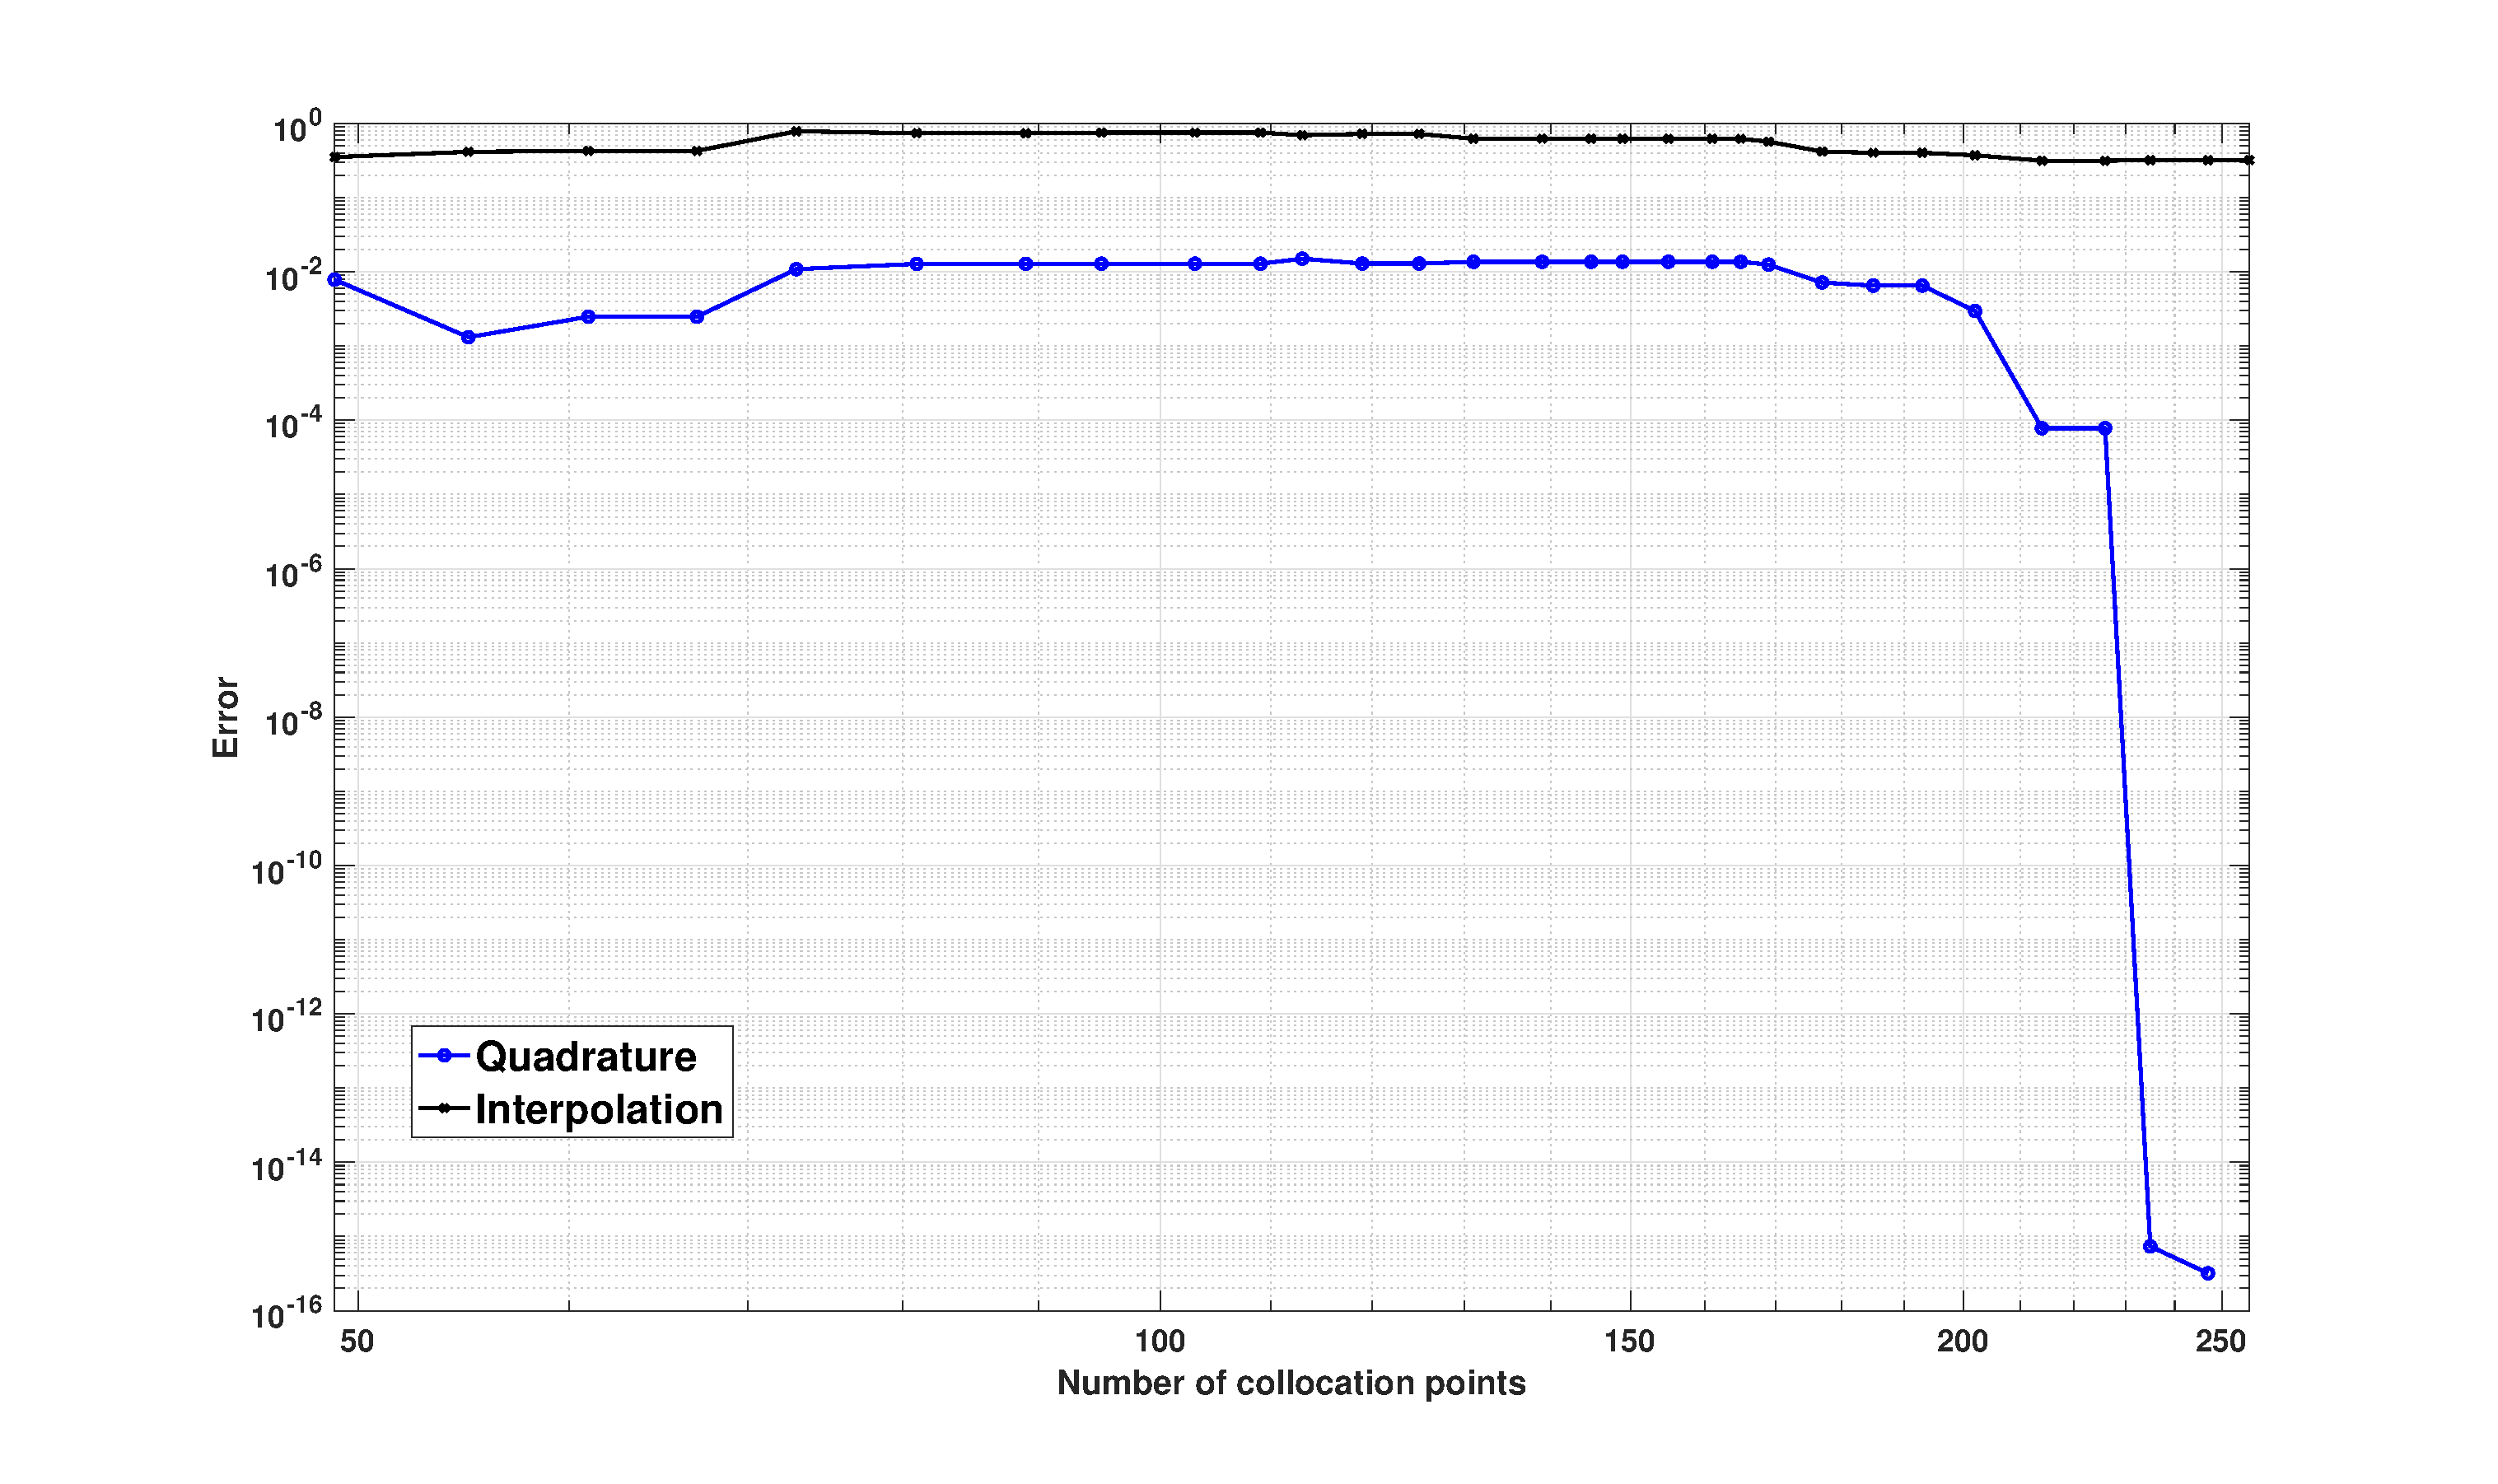
\includegraphics[width=\linewidth]{./case_N_2.eps}
		\caption{}
		\label{fig:1}
	\end{subfigure}\hfil % <-- added
	\begin{subfigure}{0.6\textwidth}
		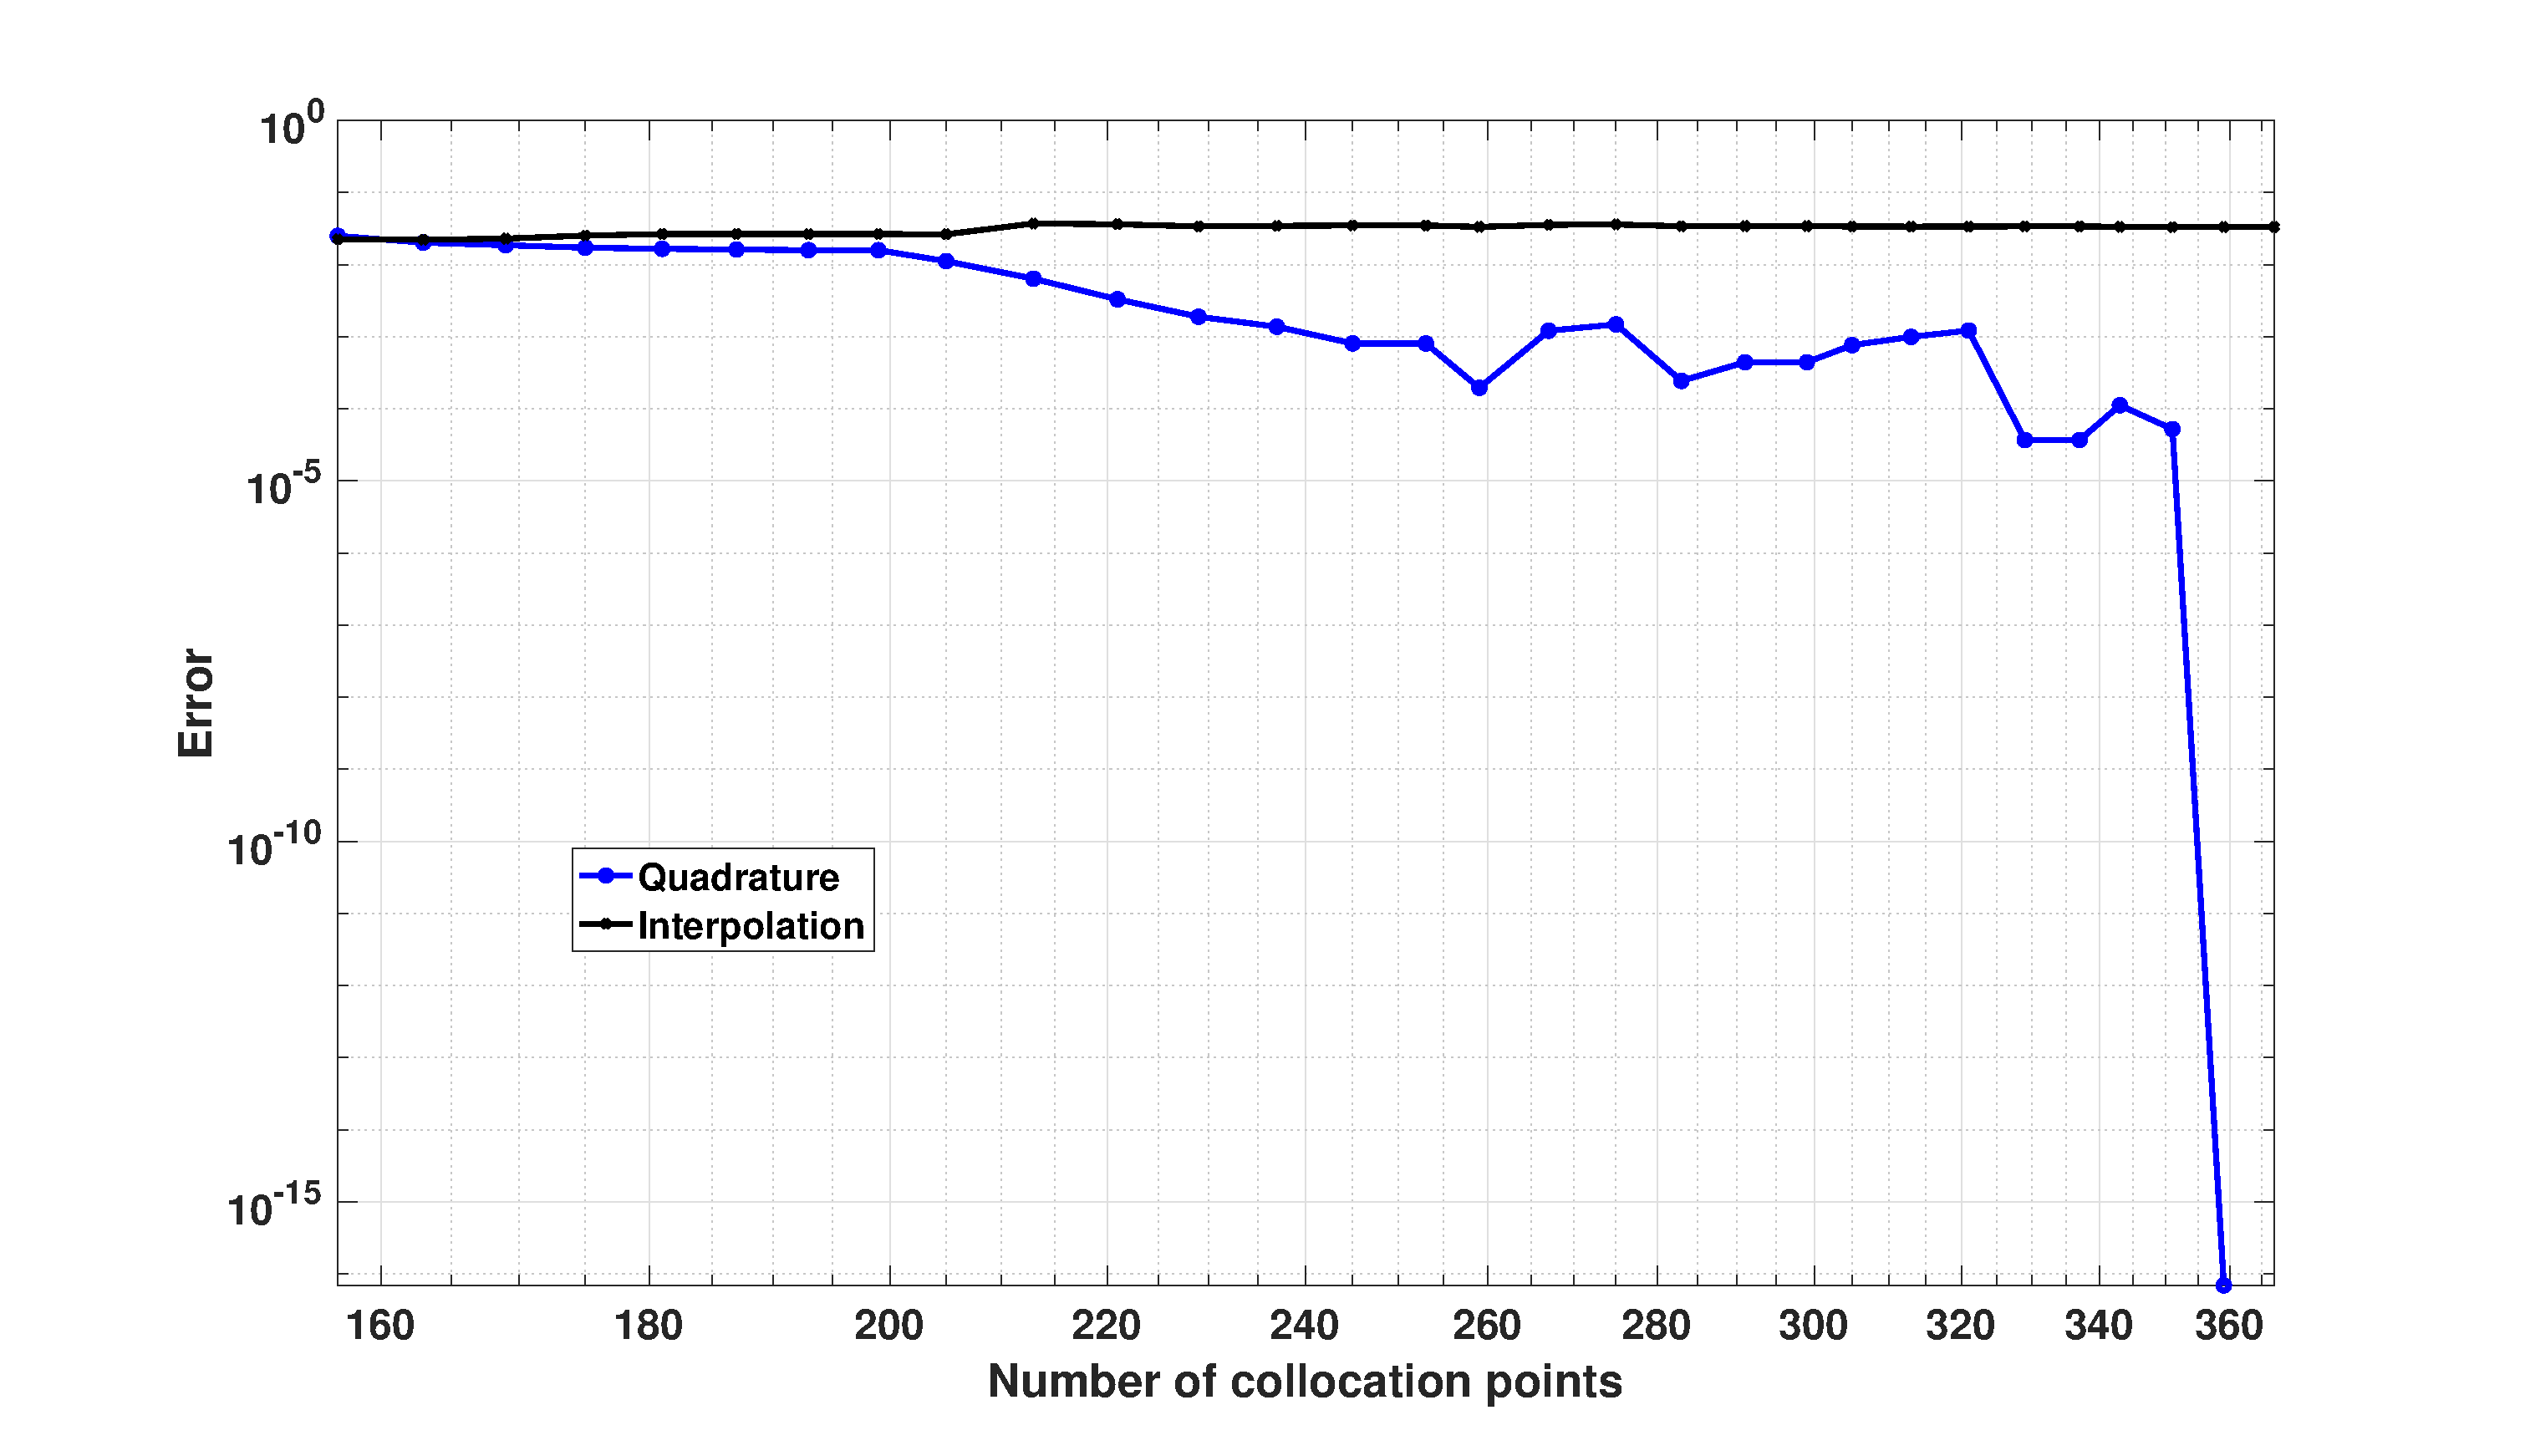
\includegraphics[width=\linewidth]{./case_N_4.eps}
		\caption{}
		\label{fig:2}
	\end{subfigure}\hfil % <-- added
	\begin{subfigure}{0.6\textwidth}
		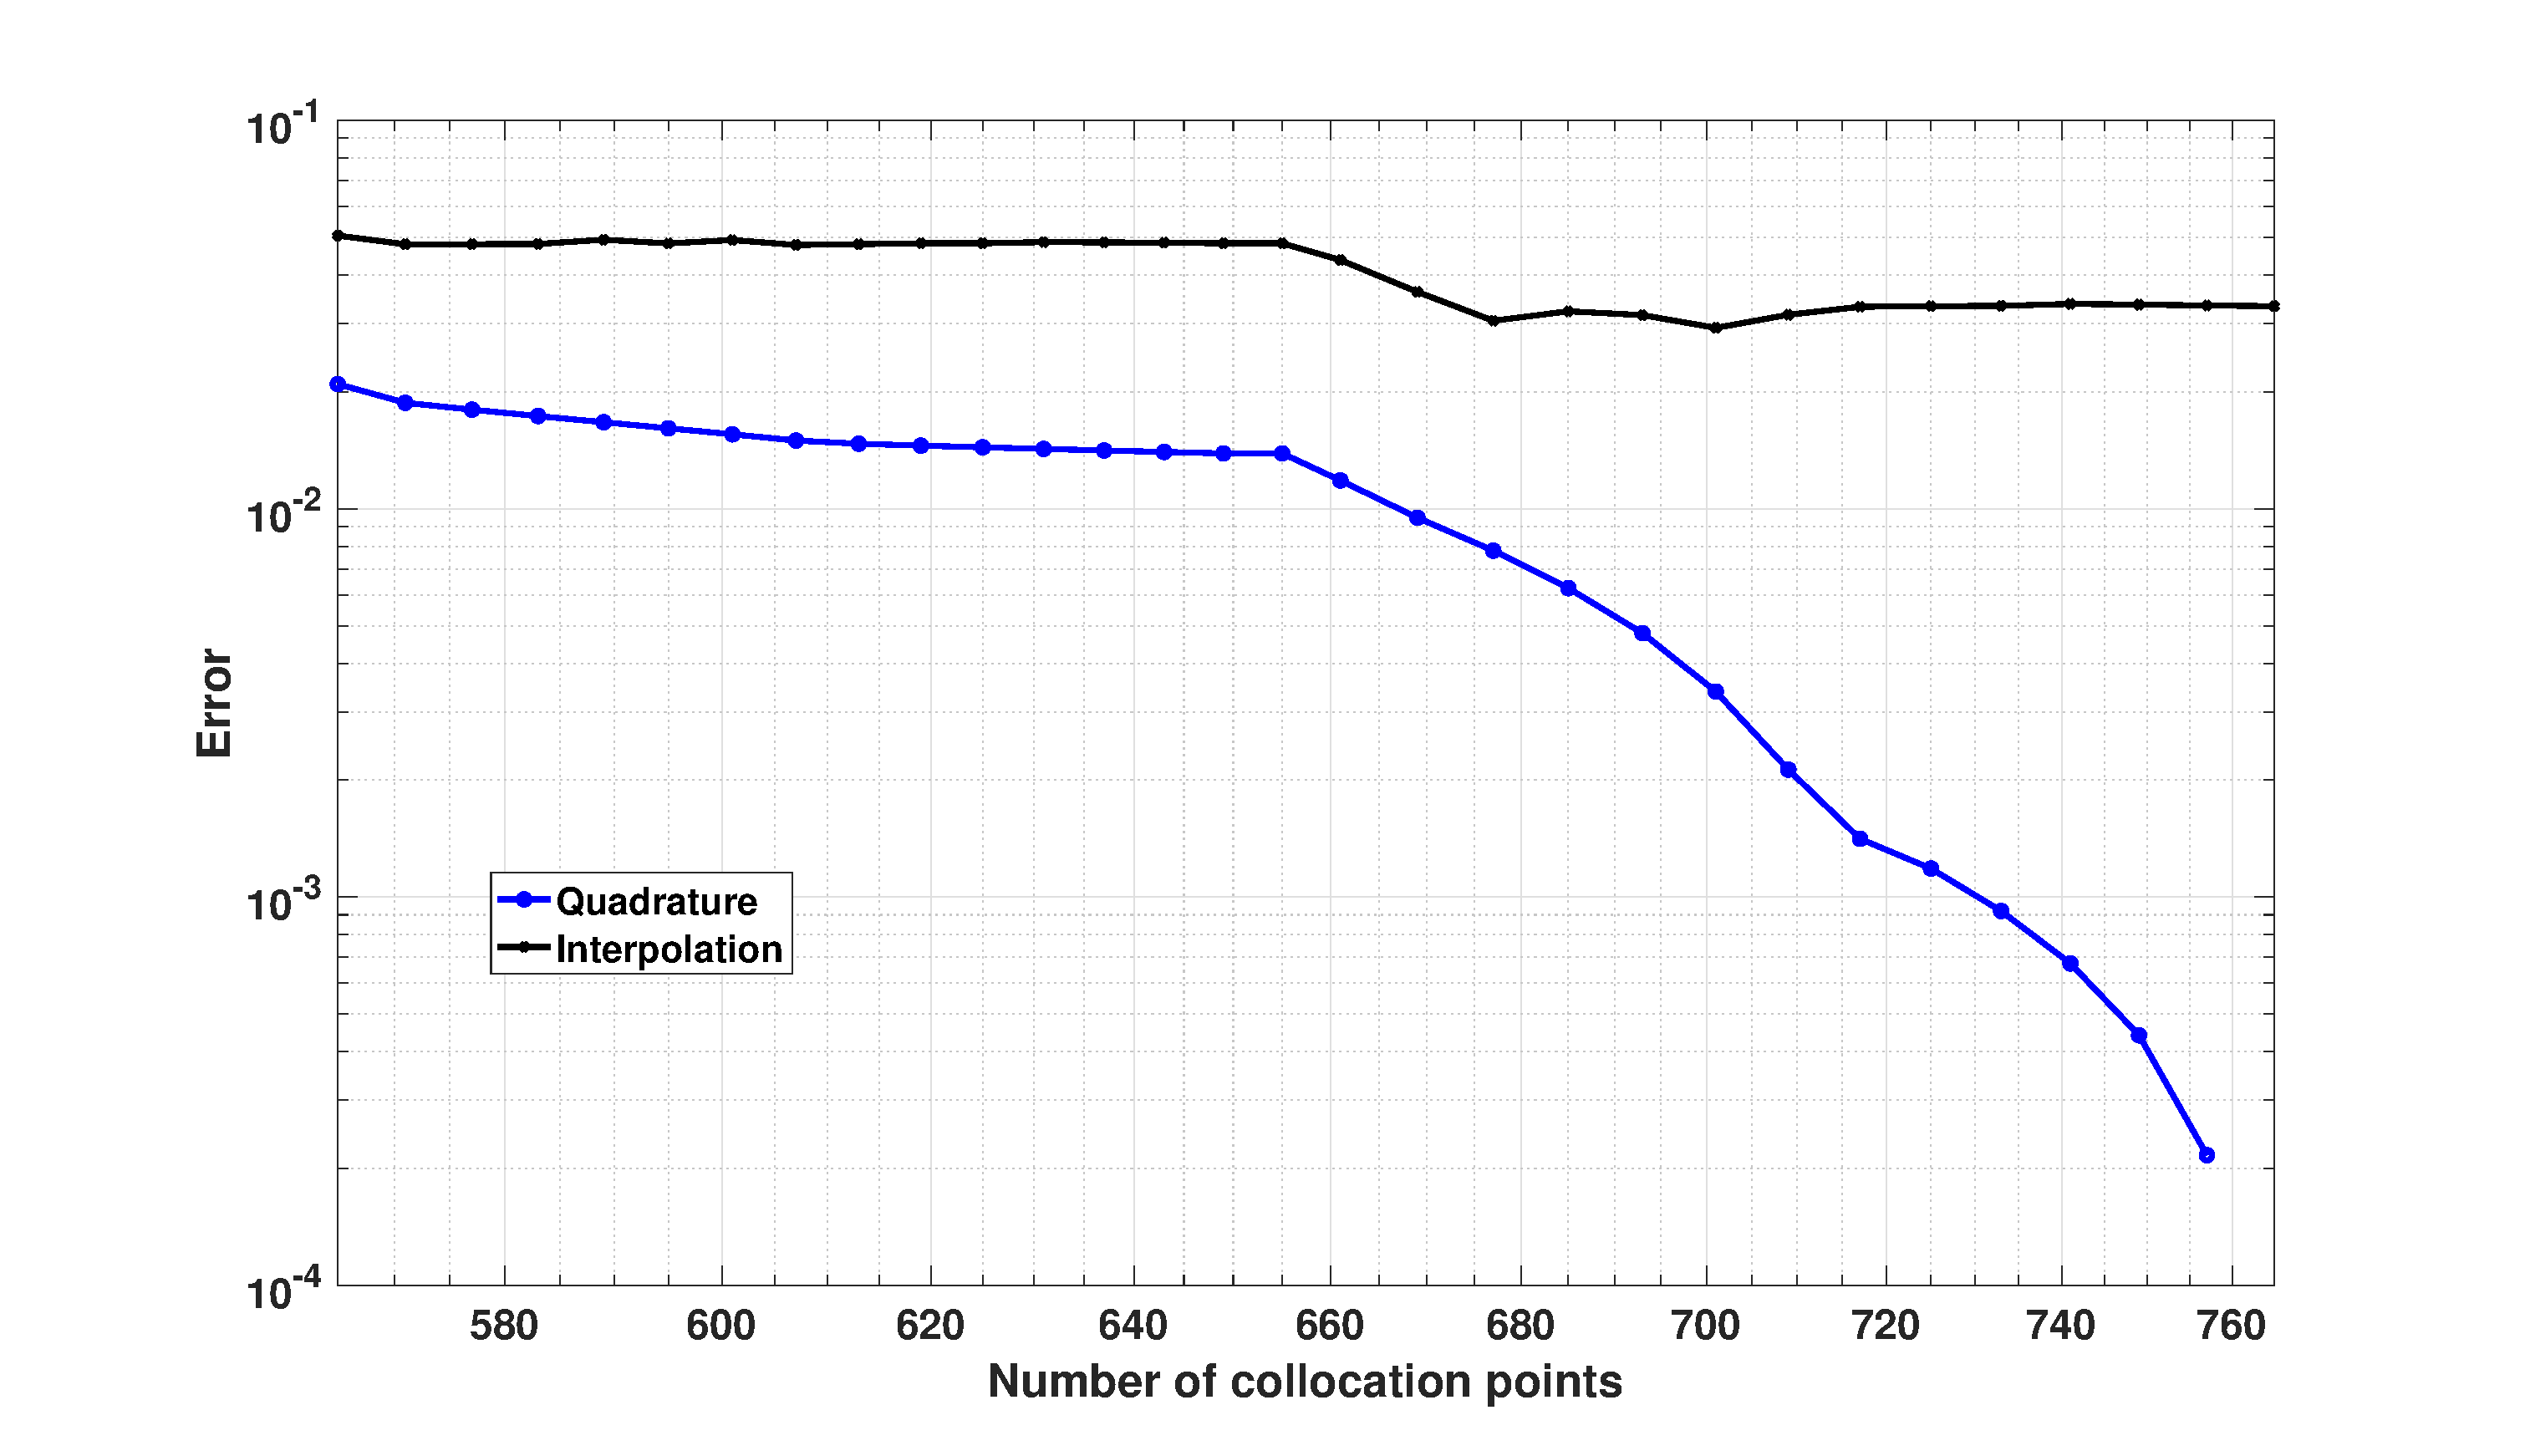
\includegraphics[width=\linewidth]{./case_N_8.eps}
		\caption{}
		\label{fig:3}
	\end{subfigure}
	\caption{Quadrature (computed as the difference between the quadrature solution and a reference solution computed with very high number of quadrature points),   and interpolation error  (as explained in the first way of Section \ref{sec:MISC error estimate}) for $3$ different cases of number of time steps: a) $N=2$, b) $N=4$,  c) $N=8$}
	\label{fig:Quadrature and interpolation error estimation for 3 different cases of number of time steps}
\end{figure}
\FloatBarrier



 %%%%%%%%%%%%%%%%%%%%%%%%%%%%%%%%%%%%%%%%%%
%References
%%%%%%%%%%%%%%%%%%%%%%%%%%%%%%%%%%%%%%%%%%

\bibliographystyle{plain}
\bibliography{smoothing_rBergomi.bib} 








 

 

 
 
 


\end{document}